\documentclass[11pt,a4paper]{article}

% ── Packages ──────────────────────────────────────────────────────────────────
\usepackage{amsmath, amssymb, amsthm}
\usepackage{geometry}
\usepackage{graphicx}
\usepackage{xcolor}
\usepackage{tikz}
\usepackage{pgfplots}
\usepackage{bm}
\usepackage{hyperref}
\usepackage{booktabs}
\usepackage{caption}
\usepackage{mathtools}
\usepackage{cleveref}

\usetikzlibrary{arrows.meta, angles, quotes, calc, decorations.pathreplacing,
                decorations.markings, patterns, positioning}
\pgfplotsset{compat=1.18}

\geometry{margin=2.5cm}
\hypersetup{colorlinks=true, linkcolor=blue, citecolor=blue, urlcolor=blue}

% ── Convenience macros ────────────────────────────────────────────────────────
\newcommand{\R}{\mathbb{R}}
\newcommand{\dpdt}[1]{\dot{p}_{#1}}
\newcommand{\dpdx}[1]{\dot{p}_{x,#1}}
\newcommand{\dpdy}[1]{\dot{p}_{y,#1}}
\newcommand{\vmax}{v_{\max}}
\newcommand{\wmax}{\omega_{\max}}

% ─────────────────────────────────────────────────────────────────────────────
\title{\textbf{Single-Integrator to Unicycle Velocity Conversion}\\[4pt]
       \large Mathematical Derivation and Implementation Notes}
\author{Multi-Robot Formation Control — ArUco Real-World Edition}
\date{\today}

\begin{document}
\maketitle
\tableofcontents
\vspace{1em}

% =============================================================================
\section{Overview}
% =============================================================================

The Double-Angle Visual Cone CBF controller produces \emph{single-integrator}
velocity commands
\[
  \dpdt{i} = \begin{bmatrix}\dpdx{i}\\\dpdy{i}\end{bmatrix} \in \R^2
\]
for each robot~$i$.  Physical TurtleBot3 robots, however, are
\emph{unicycle} systems commanded via linear speed~$v_i$ and angular
speed~$\omega_i$.  This document derives the transformation that converts
$\dpdt{i}$ into $(v_i,\,\omega_i)$ and documents the implementation
choices made in \texttt{multi\_unicycle\_controller.py}.

% =============================================================================
\section{Unicycle Kinematic Model}
% =============================================================================

A unicycle robot at configuration $(x_i,\,y_i,\,\theta_i)$ obeys
\begin{equation}\label{eq:unicycle}
  \begin{bmatrix}\dot x_i\\\dot y_i\\\dot\theta_i\end{bmatrix}
  =
  \begin{bmatrix}\cos\theta_i & 0\\\sin\theta_i & 0\\ 0 & 1\end{bmatrix}
  \begin{bmatrix}v_i\\\omega_i\end{bmatrix},
\end{equation}
where $v_i\in\R$ is the \emph{linear} (forward) speed and
$\omega_i\in\R$ is the \emph{angular} speed.

\begin{figure}[h]
\centering
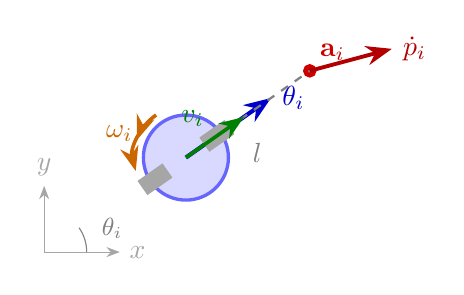
\begin{tikzpicture}[>=Stealth, thick, scale=1.2]
  % ── Robot body ──────────────────────────────────────────────────────────
  \def\cx{0}  \def\cy{0}   % robot centre
  \def\ang{35}              % heading angle (degrees)
  \def\ell{1.6}             % look-ahead distance

  % Robot circle
  \filldraw[fill=blue!15, draw=blue!60, line width=1.2pt]
      (\cx,\cy) circle (0.45);

  % Robot heading arrow
  \draw[->, blue!80!black, line width=1.5pt]
      (\cx,\cy) -- ++(\ang:1.1) node[right, blue!80!black]{$\theta_i$};

  % Wheels (two small rectangles)
  \begin{scope}[rotate around={\ang:(\cx,\cy)}]
    \filldraw[gray!70] (-0.55,-0.08) rectangle (-0.25,0.08);
    \filldraw[gray!70] ( 0.25,-0.08) rectangle ( 0.55,0.08);
  \end{scope}

  % Look-ahead point
  \coordinate (A) at ($({\cx},{\cy})+(\ang:\ell)$);
  \filldraw[red!80!black] (A) circle (0.06)
      node[above right, red!80!black]{$\mathbf{a}_i$};

  % Dashed line from centre to look-ahead
  \draw[dashed, gray, line width=0.8pt] (\cx,\cy) -- (A);
  \node[gray, below] at ($({\cx},{\cy})!0.5!(A)+(0.1,-0.2)$) {$l$};

  % Single-integrator velocity arrow at look-ahead point
  \draw[->, red!70!black, line width=1.4pt]
      (A) -- ++({\ang-20}:0.9)
      node[right, red!70!black]{$\dpdt{i}$};

  % Velocity components v and omega
  \draw[->, green!50!black, line width=1.3pt]
      (\cx,\cy) -- ++(\ang:0.75)
      node[midway, above left, green!50!black]{$v_i$};
  \draw[->, orange!80!black, line width=1.3pt,
        decoration={markings, mark=at position 0.5 with {\arrow{Stealth}}},
        postaction=decorate]
      (\cx,\cy)++({\ang+90}:0.55) arc[start angle={\ang+90},
                                       end angle={\ang+160}, radius=0.55];
  \node[orange!80!black] at ($({\cx},{\cy})+({\ang+125}:0.75)$)
      {$\omega_i$};

  % World-frame axes
  \draw[->, gray!70, thin] (-1.5,-1.0) -- (-0.7,-1.0)
      node[right, gray!70]{$x$};
  \draw[->, gray!70, thin] (-1.5,-1.0) -- (-1.5,-0.3)
      node[above, gray!70]{$y$};

  % Angle arc
  \draw[gray, thin] (-1.5+0.45,-1.0) arc[start angle=0,
       end angle=\ang, radius=0.45];
  \node[gray, right] at (-1.5+0.5,-0.75) {\small$\theta_i$};
\end{tikzpicture}
\caption{Unicycle robot with centre~$(x_i,y_i)$, heading~$\theta_i$,
         linear speed~$v_i$, angular speed~$\omega_i$, and look-ahead
         point~$\mathbf{a}_i$ at distance~$l$ along the heading axis.
         The single-integrator velocity~$\dpdt{i}$ is prescribed at
         $\mathbf{a}_i$.}
\label{fig:unicycle}
\end{figure}

% =============================================================================
\section{Look-Ahead Point Construction}
% =============================================================================

To make the unicycle system amenable to single-integrator design, we
introduce a \emph{look-ahead} (auxiliary) point~$\mathbf{a}_i$ located a
distance~$l>0$ ahead of the robot along its heading:
\begin{equation}\label{eq:lookahead_pos}
  \mathbf{a}_i
  = \begin{bmatrix}x_i + l\cos\theta_i\\ y_i + l\sin\theta_i\end{bmatrix}.
\end{equation}

\noindent Differentiating with respect to time and substituting
\eqref{eq:unicycle}:
\begin{align}
  \dot a_{x,i} &= \dot x_i - l\sin\theta_i\,\dot\theta_i
               = v_i\cos\theta_i - l\sin\theta_i\,\omega_i, \label{eq:adot_x}\\
  \dot a_{y,i} &= \dot y_i + l\cos\theta_i\,\dot\theta_i
               = v_i\sin\theta_i + l\cos\theta_i\,\omega_i. \label{eq:adot_y}
\end{align}

In matrix form:
\begin{equation}\label{eq:forward}
  \underbrace{\begin{bmatrix}\dot a_{x,i}\\\dot a_{y,i}\end{bmatrix}}_{\dpdt{i}}
  =
  \underbrace{\begin{bmatrix}
    \cos\theta_i & -l\sin\theta_i \\
    \sin\theta_i & \phantom{-}l\cos\theta_i
  \end{bmatrix}}_{M(\theta_i,l)}
  \begin{bmatrix}v_i\\\omega_i\end{bmatrix}.
\end{equation}

% =============================================================================
\section{Inversion: Unicycle Commands from Single-Integrator Velocity}
% =============================================================================

\subsection{Invertibility}

The determinant of $M(\theta_i,l)$ is
\begin{equation}
  \det M = l\cos^2\theta_i + l\sin^2\theta_i = l > 0
  \quad \forall\,\theta_i,\; l\neq 0,
\end{equation}
so $M$ is always invertible for any non-zero look-ahead distance.

\subsection{Closed-Form Inverse}

Using the formula for a $2\times 2$ inverse:
\begin{equation}\label{eq:Minv}
  M^{-1}(\theta_i,l)
  = \frac{1}{l}
    \begin{bmatrix}
      l\cos\theta_i  & l\sin\theta_i \\
      -\sin\theta_i  & \cos\theta_i
    \end{bmatrix}
  = \begin{bmatrix}
      \cos\theta_i          & \sin\theta_i \\
      -\dfrac{\sin\theta_i}{l} & \dfrac{\cos\theta_i}{l}
    \end{bmatrix}.
\end{equation}

\noindent Therefore the unicycle commands that realise any desired
single-integrator velocity $\dpdt{i}$ are
\begin{equation}\label{eq:exact_conversion}
  \boxed{
  \begin{bmatrix}v_i\\\omega_i\end{bmatrix}
  = M^{-1}(\theta_i,l)\,\dpdt{i}
  = \begin{bmatrix}
      \cos\theta_i\,\dpdx{i} + \sin\theta_i\,\dpdy{i}\\[6pt]
      \dfrac{-\sin\theta_i\,\dpdx{i} + \cos\theta_i\,\dpdy{i}}{l}
    \end{bmatrix}.}
\end{equation}

% =============================================================================
\section{Implementation in Code}
% =============================================================================

\subsection{Linear velocity gain}

The implementation uses a gain of~$2$ on~$v_i$:
\begin{equation}\label{eq:impl_v}
  v_i = 2\bigl(\dpdx{i}\cos\theta_i + \dpdy{i}\sin\theta_i\bigr).
\end{equation}
This effectively scales the CBF output by a factor of~$2$ in the
forward-speed direction, increasing responsiveness without affecting angular
convergence (the $\omega_i$ formula is unchanged from \eqref{eq:exact_conversion}).

\subsection{Angular velocity}

\begin{equation}\label{eq:impl_w}
  \omega_i
  = \frac{-\dpdx{i}\sin\theta_i + \dpdy{i}\cos\theta_i}{l},
  \qquad l = 0.1\;\text{m.}
\end{equation}

\subsection{Compact matrix form}

Combining \eqref{eq:impl_v} and \eqref{eq:impl_w}:
\begin{equation}\label{eq:T}
  \begin{bmatrix}v_i\\\omega_i\end{bmatrix}
  =
  \underbrace{\begin{bmatrix}
    2\cos\theta_i & 2\sin\theta_i \\[4pt]
    -\dfrac{\sin\theta_i}{l} & \dfrac{\cos\theta_i}{l}
  \end{bmatrix}}_{T(\theta_i)}
  \begin{bmatrix}\dpdx{i}\\\dpdy{i}\end{bmatrix}.
\end{equation}

\subsection{Velocity saturation}

To respect physical actuator limits, both commands are clipped:
\begin{align}
  v_i      &\leftarrow \operatorname{clip}(v_i,\,-\vmax,\,+\vmax),
            \qquad \vmax = 0.18\;\text{m/s}, \label{eq:sat_v}\\
  \omega_i &\leftarrow \operatorname{clip}(\omega_i,\,-\wmax,\,+\wmax),
            \qquad \wmax = 1.50\;\text{rad/s}. \label{eq:sat_w}
\end{align}

% =============================================================================
\section{Signal Flow Diagram}
% =============================================================================

\begin{figure}[ht]
\centering
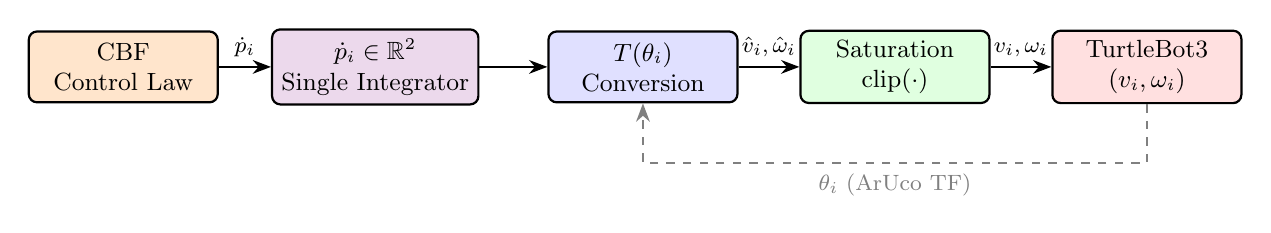
\begin{tikzpicture}[>=Stealth, thick,
    myblock/.style={draw, rounded corners=3pt, minimum width=2.4cm,
                    minimum height=0.9cm, align=center, font=\small},
    arr/.style={->, thick}]

  % Nodes placed at explicit x positions
  \node[myblock, fill=orange!20]      (cbf) at (0,0)   {CBF\\Control Law};
  \node[myblock, fill=violet!15]      (si)  at (3.2,0) {$\dpdt{i}\in\R^2$\\Single Integrator};
  \node[myblock, fill=blue!12]        (T)   at (6.6,0) {$T(\theta_i)$\\Conversion};
  \node[myblock, fill=green!12]       (sat) at (9.8,0) {Saturation\\$\mathrm{clip}(\cdot)$};
  \node[myblock, fill=red!12]         (bot) at (13.0,0){TurtleBot3\\$(v_i,\omega_i)$};

  % Forward arrows
  \draw[arr] (cbf) -- (si)  node[midway, above, font=\footnotesize]{$\dot p_i$};
  \draw[arr] (si)  -- (T);
  \draw[arr] (T)   -- (sat) node[midway, above, font=\footnotesize]{$\hat v_i,\hat\omega_i$};
  \draw[arr] (sat) -- (bot) node[midway, above, font=\footnotesize]{$v_i,\omega_i$};

  % theta feedback arrow (below)
  \draw[arr, gray, dashed]
      (bot.south) -- ++(0,-0.75) -| (T.south)
      node[near start, below, font=\footnotesize, gray]{$\theta_i$ (ArUco TF)};

\end{tikzpicture}
\caption{Signal flow for robot~$i$. The CBF law outputs a single-integrator
velocity~$\dpdt{i}$; the look-ahead transformation~$T(\theta_i)$ converts it
to unicycle commands; saturation enforces actuator limits; the robot executes
$(v_i,\omega_i)$.  The heading~$\theta_i$ is fed back from the ArUco TF2
measurement.}
\label{fig:flow}
\end{figure}

% =============================================================================
\section{Parameter Summary}
% =============================================================================

\begin{table}[h]
\centering
\caption{Parameters used in the unicycle conversion.}
\begin{tabular}{llll}
\toprule
\textbf{Symbol} & \textbf{Variable in code} & \textbf{Value} & \textbf{Description}\\
\midrule
$l$       & \texttt{self.length}     & $0.10\;\text{m}$     & Look-ahead distance\\
$\vmax$   & \texttt{self.v\_max}     & $0.18\;\text{m/s}$   & Max linear speed\\
$\wmax$   & \texttt{self.omega\_max} & $1.50\;\text{rad/s}$ & Max angular speed\\
$v$-gain  & (hardcoded)              & $2$                  & Extra linear gain\\
\bottomrule
\end{tabular}
\label{tab:params}
\end{table}

% =============================================================================
\section{Geometric Interpretation}
% =============================================================================

\begin{figure}[h]
\centering
% --- All coordinates are fixed numbers (heading=30deg, look-ahead=1.1) ---
% A = look-ahead point at (1.1*cos30, 1.1*sin30) = (0.953, 0.55)
% SI velocity direction: 60 deg, length 0.85
%   tip P = A + 0.85*(cos60, sin60) = (0.953+0.425, 0.55+0.736) = (1.378, 1.286)
% Forward projection (onto 30-deg axis) of the SI vector:
%   proj = 0.85*cos(60-30) = 0.85*cos30 = 0.736
%   Fwd endpoint F = A + 0.736*(cos30,sin30) = (0.953+0.637, 0.55+0.368) = (1.590, 0.918)
% Lateral projection (perp to 30-deg, i.e. 120-deg axis):
%   perp = 0.85*sin(60-30) = 0.85*sin30 = 0.425
%   Lat endpoint L = A + 0.425*(cos120,sin120) = (0.953-0.213, 0.55+0.368) = (0.740, 0.918)
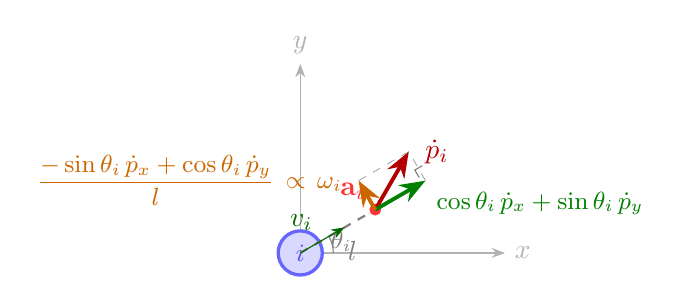
\begin{tikzpicture}[>=Stealth, thick]
  % World axes
  \draw[->, gray!60, thin] (0,0) -- (2.6,0) node[right, gray!60]{$x$};
  \draw[->, gray!60, thin] (0,0) -- (0,2.4) node[above, gray!60]{$y$};

  % Robot
  \filldraw[fill=blue!15, draw=blue!60, line width=1.2pt] (0,0) circle (0.28);
  \node[blue!70] at (0,0) {\small$i$};

  % Heading axis (30 deg)
  \draw[blue!50, dashed, thin] (0,0) -- (30:1.8);

  % Look-ahead point A
  \coordinate (A) at (30:1.1);
  \draw[gray, dashed] (0,0) -- (A);
  \filldraw[red!80] (A) circle (0.06);
  \node[above left, red!80] at (A) {$\mathbf{a}_i$};
  \node[gray, below right] at ($(0,0)!0.5!(A)$) {$l$};

  % SI velocity vector: from A at 60 deg, length 0.85
  \coordinate (P) at (1.378, 1.286);  % tip of SI vector
  \draw[->, red!70!black, line width=1.4pt]
      (A) -- (P)
      node[right=2pt, red!70!black]
          {$\dpdt{i}$};

  % Forward projection F (along 30-deg heading)
  \coordinate (F) at (1.590, 0.918);
  \draw[->, green!50!black, line width=1.4pt] (A) -- (F)
      node[below right, green!50!black, font=\small]
          {$\cos\theta_i\,\dot p_{x}+\sin\theta_i\,\dot p_{y}$};

  % Lateral projection L (along 120-deg, perp to heading)
  \coordinate (L) at (0.740, 0.918);
  \draw[->, orange!80!black, line width=1.4pt] (A) -- (L)
      node[left=2pt, orange!80!black, font=\small]
          {$\dfrac{-\sin\theta_i\,\dot p_{x}+\cos\theta_i\,\dot p_{y}}{l}\,\propto\,\omega_i$};

  % Dashed completion lines (parallelogram)
  \draw[gray, very thin, dashed] (F) -- (P) -- (L);

  % Right-angle mark at F
  \draw[gray, thin] ($(F)+(-0.08,0.04)$) -- ++(120:0.11) -- ++(30:0.11);

  % Heading angle arc
  \draw[gray, thin] (0.42,0) arc[start angle=0, end angle=30, radius=0.42];
  \node[gray] at (0.52, 0.15) {\small$\theta_i$};

  % Labels: v_i direction
  \draw[->, green!40!black, thin] (0,0) -- (30:0.65)
      node[midway, above left, green!40!black]{$v_i$};
\end{tikzpicture}
\caption{Geometric decomposition of~$\dpdt{i}$ at the look-ahead
         point~$\mathbf{a}_i$ (heading $\theta_i=30^\circ$, example).
         The \textcolor{green!60!black}{green} component (parallel to heading)
         drives forward speed~$v_i$.
         The \textcolor{orange!80!black}{orange} component (perpendicular to heading),
         divided by~$l$, drives angular speed~$\omega_i$.}
\label{fig:geom}
\end{figure}

The transformation~$T(\theta_i)$ decomposes the desired single-integrator
velocity~$\dpdt{i}$ into:
\begin{enumerate}
  \item \textbf{Forward component} (parallel to heading):
        $\dpdx{i}\cos\theta_i + \dpdy{i}\sin\theta_i$
        $\;\longrightarrow\;$ proportional to~$v_i$.
  \item \textbf{Lateral component} (perpendicular to heading):
        $-\dpdx{i}\sin\theta_i + \dpdy{i}\cos\theta_i$
        $\;\longrightarrow\;$ proportional to~$\omega_i$ (scaled by~$1/l$).
\end{enumerate}
Intuitively, a large lateral error steers the robot; a large forward error
accelerates it.

% =============================================================================
\section{Complete Conversion — Step by Step}
% =============================================================================

Given the CBF output $\dpdt{i} = [\dpdx{i},\,\dpdy{i}]^\top$ and the
current ArUco heading~$\theta_i$:

\begin{enumerate}
  \item \textbf{Compute forward speed}
        \[
          \hat v_i = 2\bigl(\dpdx{i}\cos\theta_i + \dpdy{i}\sin\theta_i\bigr).
        \]
  \item \textbf{Compute angular speed}
        \[
          \hat\omega_i = \frac{-\dpdx{i}\sin\theta_i + \dpdy{i}\cos\theta_i}{l}.
        \]
  \item \textbf{Saturate}
        \[
          v_i = \operatorname{clip}(\hat v_i,\,-\vmax,\,+\vmax), \qquad
          \omega_i = \operatorname{clip}(\hat\omega_i,\,-\wmax,\,+\wmax).
        \]
  \item \textbf{Publish} $(v_i,\,\omega_i)$ as a \texttt{TwistStamped}
        message on \texttt{/bot\_\textit{i}/cmd\_vel}.
\end{enumerate}

\end{document}
